%Work Flow

%Describe the BriefCASE work flow and tools.

% Copied from DESTION paper
The BriefCASE environment provides systems engineers with a workflow and tool support for developing
products with inherent cyber-resiliency. 
\remove{In this section we provide an overview of the design, analysis, and code generation tools and how they can be used
to implement high-assurance systems.  
}

%BriefCASE is predicated on an MBSE process, in which models are the primary vehicle for
%communication and understanding among the parties tasked with designing the system. Furthermore,
%MBSE models are the primary design artifacts used for analysis, verification, testing, and code
%generation.
The  workflow starts with the development of a baseline AADL model of the system architecture
focusing on the desired functionality. This model can be analyzed using any of the existing AADL 
tools (e.g., resource usage, information flow, latency) to determine whether it is acceptable.
BriefCASE integrates additional tools that analyze the architecture model for cybersecurity vulnerabilities and
generate requirements that, when addressed, will mitigate those vulnerabilities.
These requirements are imported into the model and may be addressed using a 
collection of automated model transforms. As requirements are addressed in the design, an assurance case is updated with
corresponding evidence, computed directly from the model or by supporting analysis tools.  
Code implementing new high-assurance components as well as communication and execution infrastructure
is generated from the model along with associated assurance evidence.  

The BriefCASE tools and their interactions are shown in \figref{fig:tool-arch}.   
The following sections describe each step of the workflow in more detail, corresponding
to the tools and artifacts shown in green in the figure.  

\begin{figure*}
	\begin{center}
	  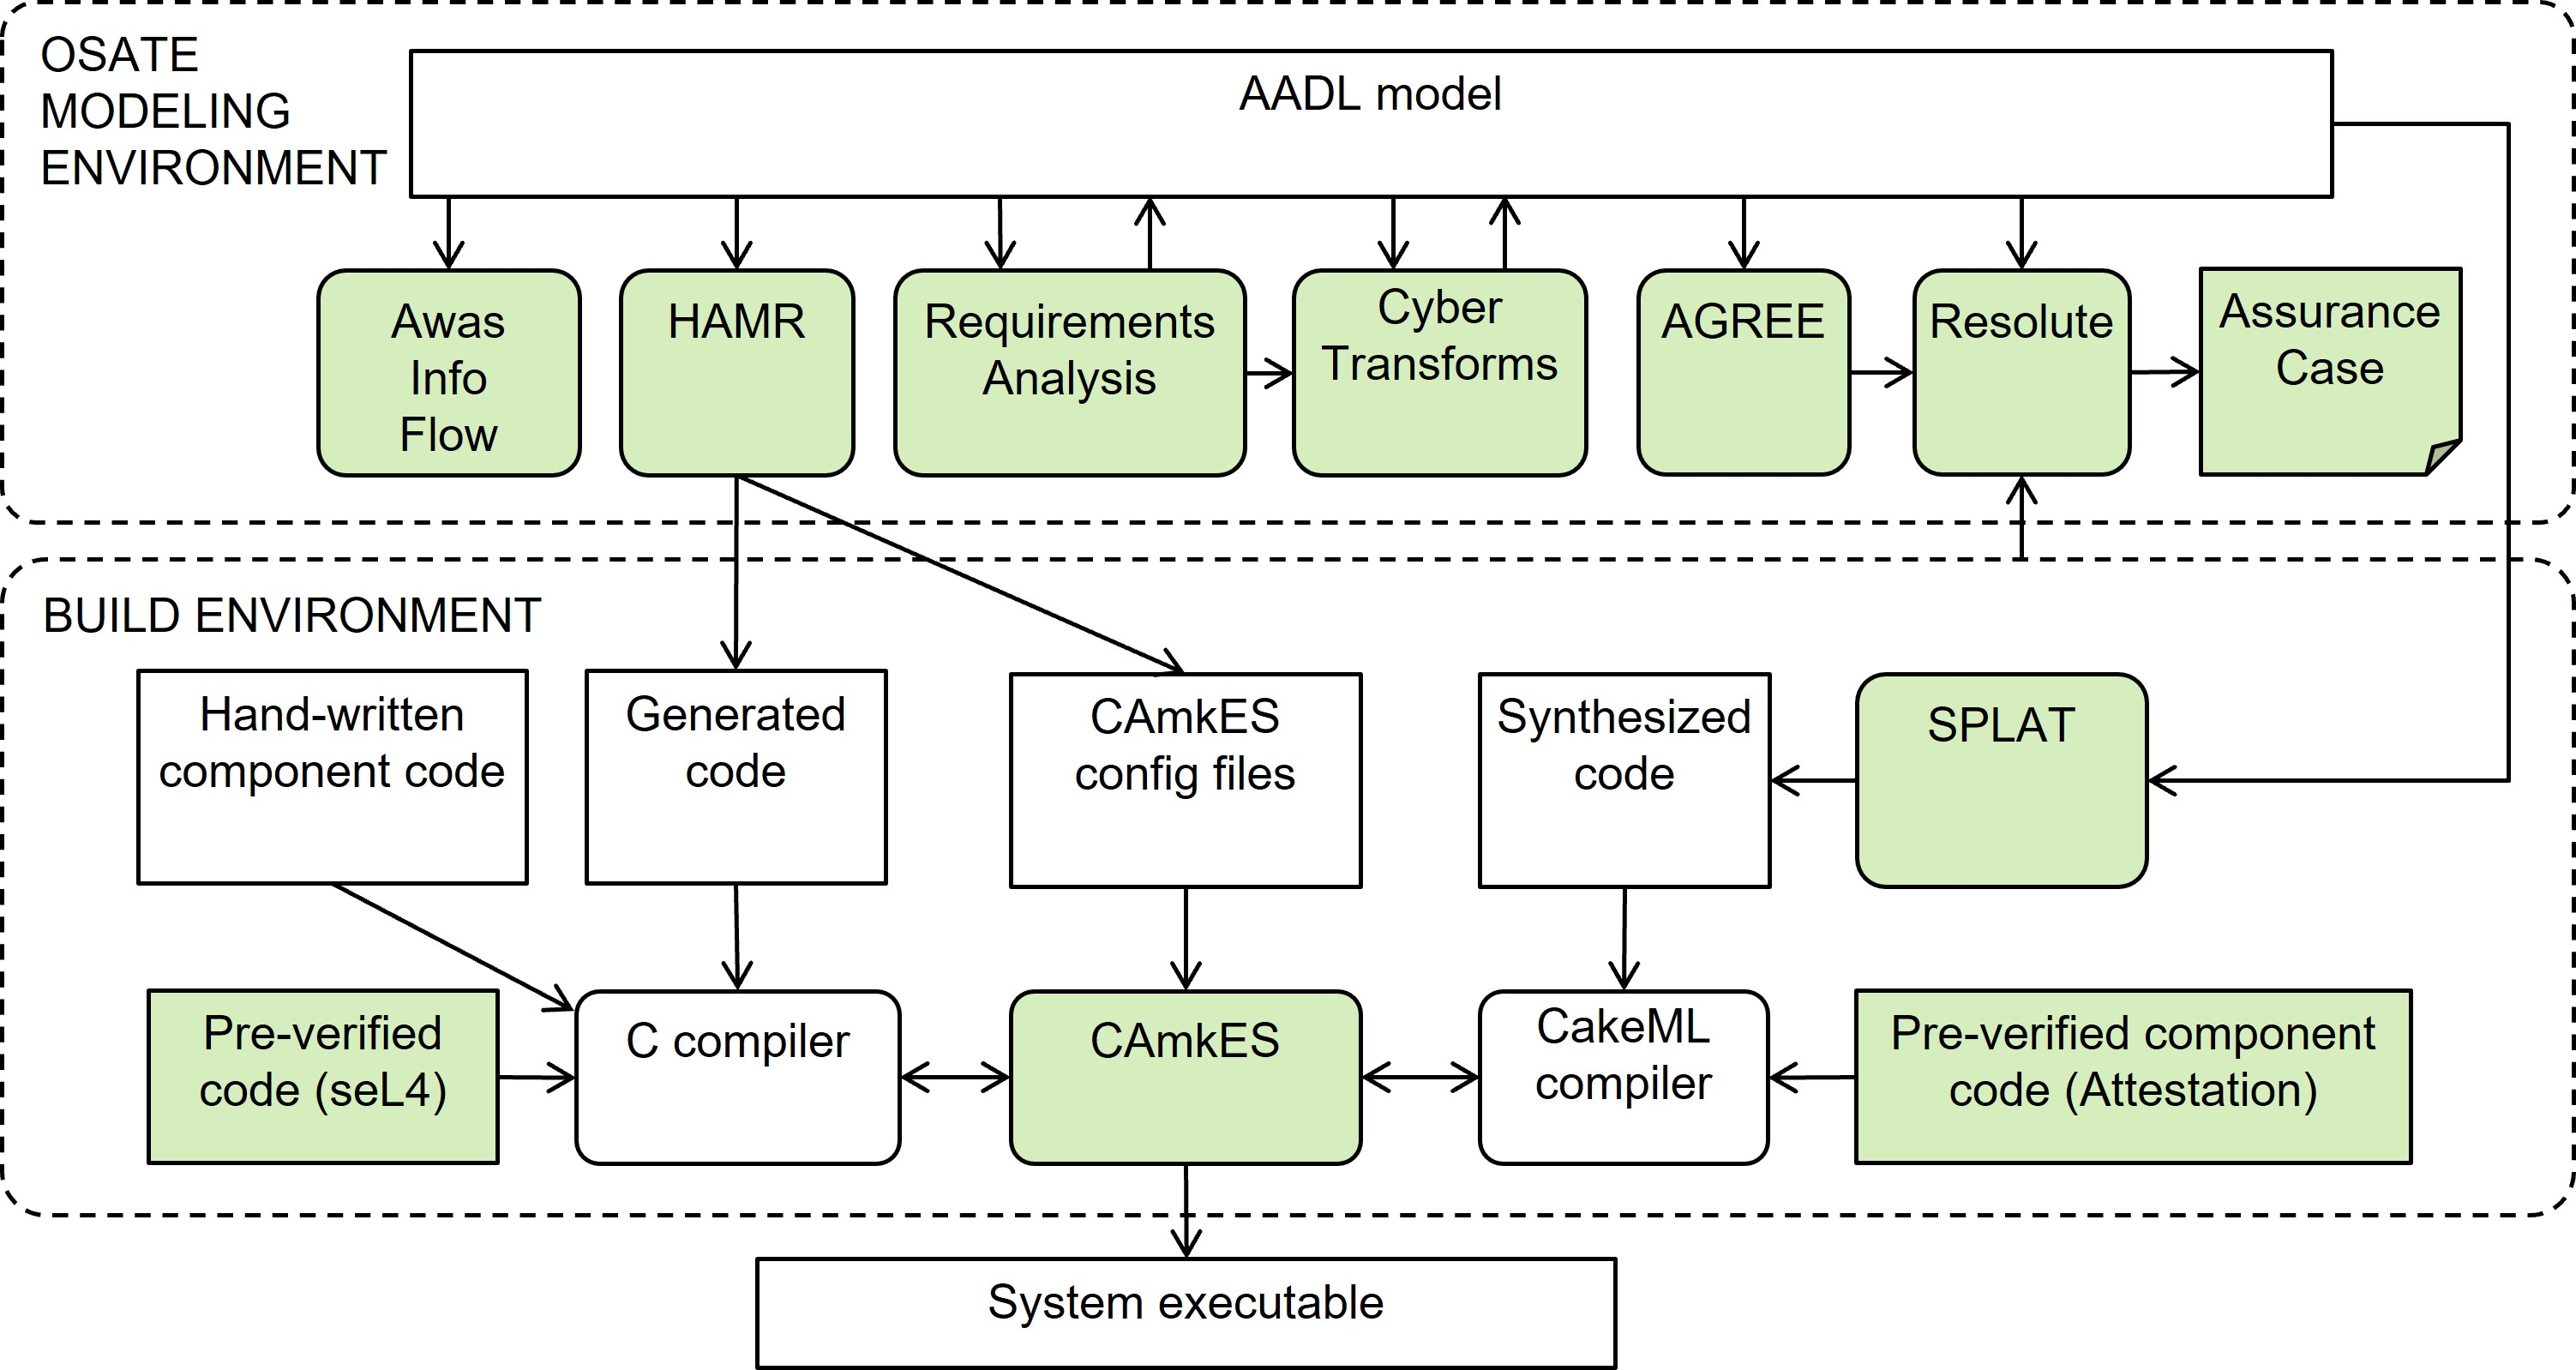
\includegraphics[width=\textwidth]{./figs/tool-arch.jpg}
  	\end{center}
	\caption{BriefCASE tool architecture.  Tools and code/artifacts discussed in the BriefCASE workflow are shown in green.} 
	\label{fig:tool-arch} 
\end{figure*}

%development process outputs, necessary
%to support the claim. In this manner, the assurance case is co-developed alongside the system
%design, and can be automatically evaluated throughout development.
